% Created 2018-05-06 Sun 21:31
\documentclass[11pt]{article}
\usepackage[utf8]{inputenc}
\usepackage[T1]{fontenc}
\usepackage{graphicx}
\usepackage{longtable}
\usepackage{hyperref}


\title{+ Title: Gene structural changes (InDels) in Chromosome 22 of dog genome were involved with Duchenne muscular dystrophy disease}
\author{Xiaotian Tang   DB1813}
\date{06 May 2018}

\begin{document}

\maketitle

\setcounter{tocdepth}{3}
\tableofcontents
\vspace*{1cm}
\begin{itemize}
\item Name: Xiaotian Tang DB1813

\begin{itemize}
\item Background

\begin{itemize}
\item Duchenne muscular dystrophy (DMD) is a severe type of muscular dystrophy. Here we have the datasets which are comparised of three conditions of dogs: 
    fast, slow and unaffected (control). For fast condition, three dog species were involved: Czar, Santana and Xerdo. For slow condition,
    there are also three dog species: Branch, Xellus and Zeus. In control, we have Bigsby and Xadius. For each dog species, we have three biological 
    replicates and three technical replicates.
\end{itemize}

\item Hypothesis: the origin of Duchenne muscular dystrophy disease is strucutre changes in multible genes.
\item Experimental procedure

\begin{itemize}
\item Merge datasets

\begin{itemize}
\item For each dog dataset, nine fastq files (three biological replicates and three technical replicates.) were merge into one big fastq file using
    ``cat'' command. The merged fastq files could be found in path:/scratch/user/tangxt/DBiology/DB1813$_{\mathrm{FinalProject}}$.data/Canis-lupus-familiaris.FinalProject.data.
\end{itemize}

\end{itemize}

\end{itemize}

\item Mapping to dog genome

\begin{itemize}
\item HISAT2 was used to map the reads of datasets to the dog genome with ``--tmo'' flag. The scripts were put in depository. The output BAM files could be found in /scratch/user/tangxt/DBiology/DB1813$_{\mathrm{FinalProject}}$.data/Hisat.data.
\end{itemize}

\item Assembling

\begin{itemize}
\item Stringtie was used to assemble the resulting mapped reads with ``-e'' flag. The scripts were put in depository. The output GTF files could be found in /scratch/user/tangxt/DBiology/DB1813$_{\mathrm{FinalProject}}$.data/stringtie.data.
     Then the GTF files were converted into GFF3 files. Meanwhile, the output eight GTF files were merged into three big GTF files as the three groups: fast, slow and unaffected using stringtie --merge tools. The three output big files 
     were further used to gffcompare. The data could be found in path /scratch/user/tangxt/DBiology/DB1813$_{\mathrm{FinalProject}}$.data/stringtie.data.
\end{itemize}

\item Annotation

\begin{itemize}
\item Before annotation, the GTF files were converted into GFF3 files using Cufflinks and gffread. MAKER was used to annotate the incorparate the
     resulting assembled transcripts. The Chromosome 22 was used as reference genome. The GFF3 files were put in est$_{\mathrm{gff}}$. In gene prediction section, augustus$_{\mathrm{species}}$
     is human. The MAKER output data could be found in path: /scratch/user/tangxt/DBiology/DB1813$_{\mathrm{FinalProject}}$.data/maker$_{\mathrm{chromosome}}$. The GFF files and transcripts files etc. files
     were generated.
\end{itemize}

\item Comparison

\begin{itemize}
\item Comparison between MAKER files

\begin{itemize}
\item After getting GFF files from MAKER annotation, gffcompare was used to compare fast vs unaffected and slow vs unaffected to get novel gene
      structure changes of fast and slow condition dog genome by using unaffected dogs as reference. The gffcompare output could be found in the path:
      /scratch/user/tangxt/DBiology/DB1813$_{\mathrm{FinalProject}}$.data/maker$_{\mathrm{chromosome}}$. The output files such as tmap, tracking, loci etc. were further used in
      tracking the genes which has novel gene structure. For example, Use the *.tmap file to extract the different transcript flags, and to extract the gene IDs,
      then use those gene IDs to locate those genes in the files.
\end{itemize}

\end{itemize}

\item Comparison between Stringtie files

\begin{itemize}
\item The Stringtie generated GTF files. As above said, the output eight GTF files were merged into three big GTF file as the three groups: fast, slow and 
      unaffected using stringtie --merge tools. Then gffcompare was used to compare fast vs unaffected and slow vs unaffected to get novel gene structure changes
      of fast and slow condition dog genome by using unaffected dogs as reference. The gffcompare output could be found in the path:
      /scratch/user/tangxt/DBiology/DB1813$_{\mathrm{FinalProject}}$.data/stringtie.data/gffcompare. The output files such as tmap, tracking, loci etc. were further used in
      tracking the genes which has novel gene structure. For example, Use the *.tmap file to extract the different transcript flags, and to extract the gene IDs,
      then use those gene IDs to locate those genes in the files.
\end{itemize}

\item IGV visualization

\begin{itemize}
\item The IGV was got from \href{https://portal.hprc.tamu.edu/pun/sys/dashboard/batch_connect/sys/igv/}{https://portal.hprc.tamu.edu/pun/sys/dashboard/batch_connect/sys/igv/}. For visualization of Maker files comparison results, the files 
     were loaded from Maker generated GFF files and annotated.gtf files. For Stringtie files comparison results visualization, the files were loaded 
     from the GTF files produced by stringtie.
\end{itemize}

\item Results

\begin{itemize}
\item Analysis of Maker outputs

\begin{itemize}
\item Unaffected VS. Fast data and Unaffected VS. Slow
\end{itemize}

\end{itemize}

\item The fast comparison file is called fast2.22.diff.out.txt, which is in the path:
   /scratch/user/tangxt/DBiology/DB1813$_{\mathrm{FinalProject}}$.data/maker$_{\mathrm{chromosome}}$/fast2vsunaffected2
\item The slow comparison file is called slow2.22.diff.out.txt, which is in the path:
   /scratch/user/tangxt/DBiology/DB1813$_{\mathrm{FinalProject}}$.data/maker$_{\mathrm{chromosome}}$/slow2vsunaffected2

\begin{itemize}
\item GFFcompare Statistics

\begin{itemize}
\item The gffcompare statistics including query mRNA, matching statistics, intron and exon data were showed in below tables. Based on gff compare of Maker outputs, I did't detect any difference for unaffected vs fast comparison. The base level, exon level, intron level of 
        Sensitivity and Precision are 100.0. However, the gene structure changes were found for unaffected vs slow condition comparison. Two novel exons,
        one missed intron, and four novel introns were identified.
\end{itemize}

\item Fast:    Query mRNAs :     449 in     421 loci  (335 multi-exon transcripts)
\item Slow:    Query mRNAs :     450 in     421 loci  (336 multi-exon transcripts)

\begin{center}
\begin{tabular}{lrrlrr}
                     &  Unaffected vs fast  &             &     &  Unaffected vs slow  &             \\
                     &         Sensitivity  &  Precision  &     &         Sensitivity  &  Precision  \\
 Base level          &               100.0  &      100.0  &     &               100.0  &       99.8  \\
 Exon level          &               100.0  &      100.0  &     &                99.8  &       99.7  \\
 Intron level        &               100.0  &      100.0  &     &                99.9  &       99.8  \\
 Intron chain level  &               100.0  &      100.0  &     &                99.4  &       99.1  \\
 Transcript level    &               100.0  &      100.0  &     &                99.6  &       99.3  \\
 Locus level         &               100.0  &      100.0  &     &                99.5  &       99.5  \\
\end{tabular}
\end{center}


\end{itemize}

\item Matching statistics

\begin{center}
\begin{tabular}{lrlr}
                         &  Unaffected vs fast  &     &  Unaffected vs slow  \\
 Matching intron chains  &                 335  &     &                 333  \\
 Matching transcripts    &                 449  &     &                 447  \\
 Matching loci           &                 421  &     &                 419  \\
\end{tabular}
\end{center}


\item Intron and Exon Data

\begin{center}
\begin{tabular}{llllll}
                 &  Unaffected vs fast  &             &     &  Unaffected vs slow  &            \\
 Missed exons    &  0/2461              &  (  0.0\%)  &     &  0/2461              &  ( 0.0\%)  \\
 Novel exons     &  0/2461              &  (  0.0\%)  &     &  2/2465              &  ( 0.1\%)  \\
 Missed introns  &  0/2010              &  (  0.0\%)  &     &  1/2010              &  ( 0.0\%)  \\
 Novel introns   &  0/2010              &  (  0.0\%)  &     &  4/2013              &  ( 0.2\%)  \\
 Missed loci:    &  0/421               &  (  0.0\%)  &     &  0/421               &  ( 0.0\%)  \\
 Novel loci:     &  0/421               &  (  0.0\%)  &     &  0/421               &  ( 0.0\%)  \\
\end{tabular}
\end{center}


\item Results (continued)

\begin{itemize}
\item Analysis of StringTie outputs
\end{itemize}

\item Unaffected VS. Fast data

\begin{itemize}
\item The fast comparison file is called fast2.22.diff.out.txt, which is in the path:
       /scratch/user/tangxt/DBiology/DB1813$_{\mathrm{FinalProject}}$.data/stringtie.data/gffcompare
\item The slow comparison file is called slow2.22.diff.out.txt, which is in the path:
       /scratch/user/tangxt/DBiology/DB1813$_{\mathrm{FinalProject}}$.data/stringtie.data/gffcompare
\end{itemize}

\item GFFcompare Statistics

\begin{itemize}
\item The gffcompare statistics including query mRNA, matching statistics, intron and exon data were showed in below tables. Based on gffcompare of StringTie 
      outputs, I did't detect any difference for unaffected and slow/fast condition dog genome.The strange thing is the intron level and missed introns. I have
      98.7 Sensitivity and Precision for intron level and my missed introns statistic is 2425/195652. Probably it is a potential bug in gffcompare. Importantly,
      I also checked the StringTie GTF files in IGV. I cannot find any difference between the three conditions, either.
\item Fast:    Query mRNAs :     38997 in     32499 loci  (31952 multi-exon transcripts)
\item Slow:    Query mRNAs :     38997 in     32499 loci  (31952 multi-exon transcripts)


\begin{center}
\begin{tabular}{lrrlrr}
                     &  Unaffected vs fast  &             &     &  Unaffected vs slow  &             \\
                     &         Sensitivity  &  Precision  &     &         Sensitivity  &  Precision  \\
 Base level          &               100.0  &      100.0  &     &               100.0  &      100.0  \\
 Exon level          &               100.0  &      100.0  &     &               100.0  &      100.0  \\
 Intron level        &                98.7  &       98.7  &     &                98.7  &       98.7  \\
 Intron chain level  &               100.0  &      100.0  &     &               100.0  &      100.0  \\
 Transcript level    &               100.0  &      100.0  &     &               100.0  &      100.0  \\
 Locus level         &               100.0  &      100.0  &     &               100.0  &      100.0  \\
\end{tabular}
\end{center}


\item Matching statistics   


\begin{center}
\begin{tabular}{lrlr}
                         &  Unaffected vs fast  &     &  Unaffected vs slow  \\
 Matching intron chains  &               31952  &     &               31952  \\
 Matching transcripts    &               38997  &     &               38997  \\
 Matching loci           &               32499  &     &               32499  \\
\end{tabular}
\end{center}


\end{itemize}

\item Intron and Exon Data


\begin{center}
\begin{tabular}{llllll}
                 &  Unaffected vs fast  &             &     &  Unaffected vs slow  &            \\
 Missed exons    &  0/234447            &  (  0.0\%)  &     &  0/234447            &  ( 0.0\%)  \\
 Novel exons     &  0/234423            &  (  0.0\%)  &     &  0/234423            &  ( 0.0\%)  \\
 Missed introns  &  2425/195652         &  (  1.2\%)  &     &  2425/195652         &  ( 1.2\%)  \\
 Novel introns   &  0/195652            &  (  0.0\%)  &     &  0/195652            &  ( 0.0\%)  \\
 Missed loci:    &  0/32499             &  (  0.0\%)  &     &  0/32499             &  ( 0.0\%)  \\
 Novel loci:     &  0/32499             &  (  0.0\%)  &     &  0/32499             &  ( 0.0\%)  \\
\end{tabular}
\end{center}


\item Results (continued)

\begin{itemize}
\item The location and annotation of the genes

\begin{itemize}
\item I mainly focused on Chromosome 22. Based on Maker analysis, no gene structure variation was found between fast and unaffected conditions dogs.
     However, I did find two genes exhibiting distinct gene structures between slow and unaffected conditions dogs. From diff.out.txt file, I could find the first gene ID is maker-22-exonerate$_{\mathrm{protein2genome\}}$-gene-293.1
     in unaffected dog genome (reference gene) and maker-22-exonerate$_{\mathrm{protein2genome\}}$-gene-293.67 in slow dog genome. The second gene ID is maker-22-exonerate$_{\mathrm{protein2genome\}}$-gene-570.2
     in unaffected dog genome (reference gene) and maker -22-exonerate$_{\mathrm{est2genome\}}$-gene-570.0 in slow dog genome. In the slow2.22.tracking file, I could grep the two gene assemble 
     IDs, which are XLOC$_{\mathrm{000301\}}$ and XLOC$_{\mathrm{000397\}}$, respectively. So then I traced the chromosome location of those two genes in the slow2.22.loci file based on the above assemble IDs. 
     The first gene is located in 22[-]29309412-29310477, and the second gene is located in 22[-]56945092-56946253. All the files were put in the path: 
     /scratch/user/tangxt/DBiology/DB1813$_{\mathrm{FinalProject}}$.data/maker$_{\mathrm{chromosome}}$/slow2vsunaffected2.
\item Due to both the two genes are exonerate$_{\mathrm{est2genome\}}$-genes, I cannot get real gene name besed on Ensembl ID. Therefore, I extracted their sequences from 22.maker.transcripts.fasta
      file, and then blasted in NCBI. Based on BLAST results, the first gene is highly identical to heterogeneous nuclear ribonucleoprotein A1 (HNRNPA1) gene. The second gene is highly
      identical to glyceraldehyde-3-phosphate dehydrogenase (GAPDH) gene. The BALST results were shown in the below figure.

     \#+CAPTION: blast of two genes in NCBI
     \#+NAME:   fig: blast of two genes in NCBI 
     \centerline{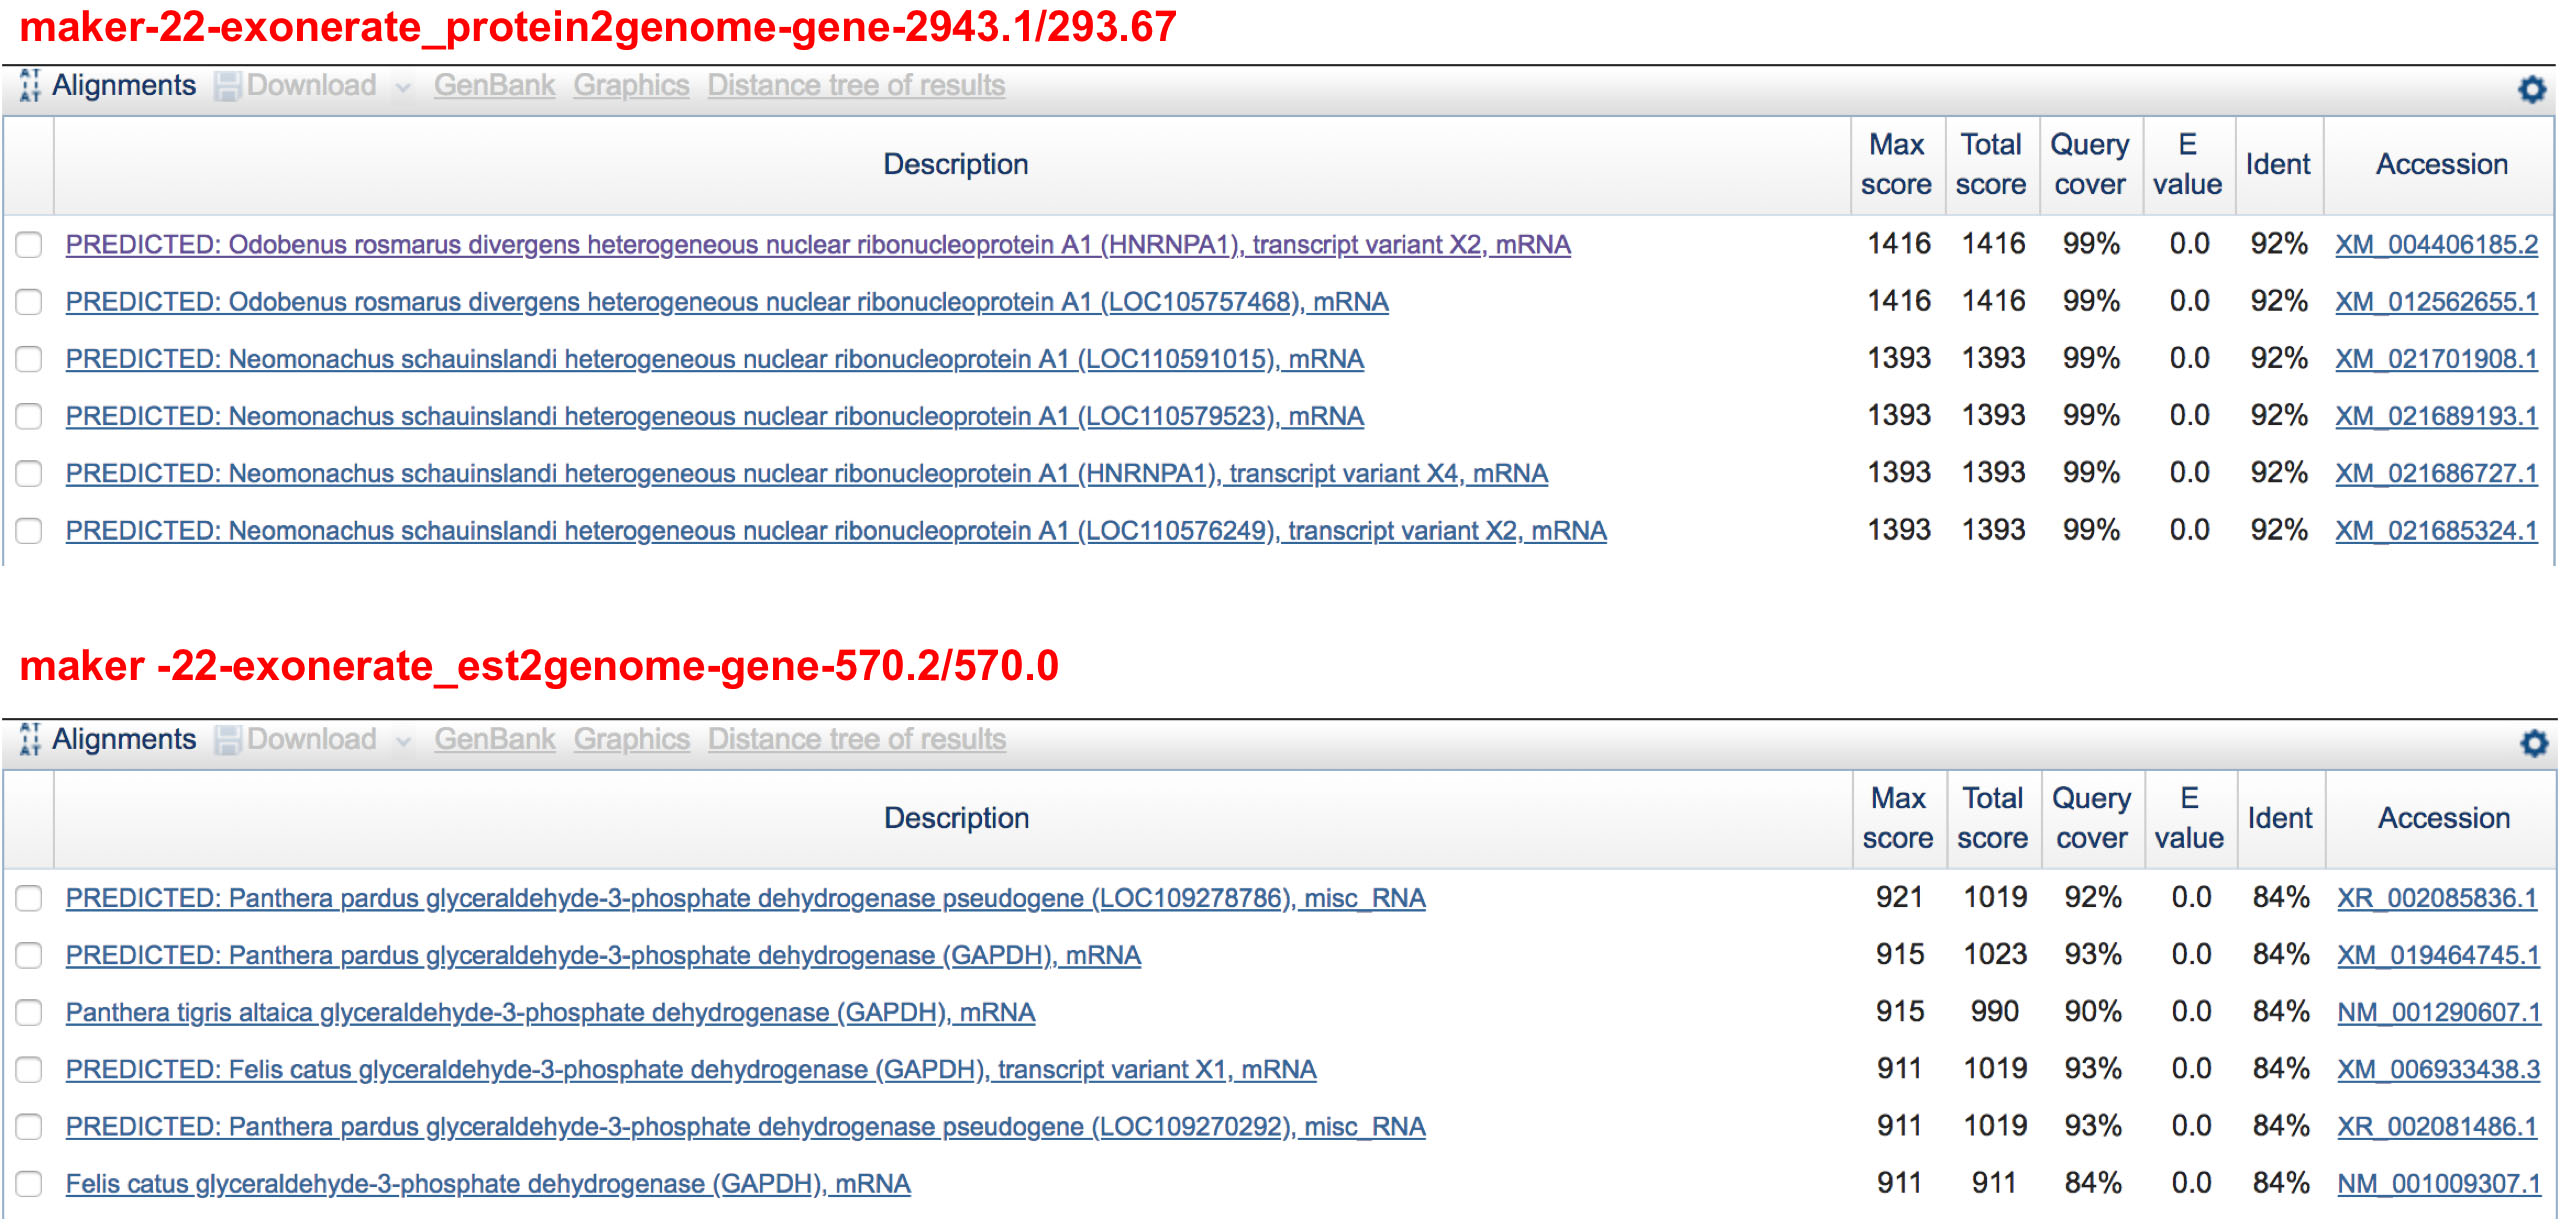
\includegraphics[width=10em]{./BLAST.jpg}}
\end{itemize}

\end{itemize}

\item Results (continued)

\begin{itemize}
\item The predicted function of the genes and implication in human disease

\begin{itemize}
\item The two genes HNRNPA1 and GAPDH have their predicted function based on Uniprot output. HNRNPA1 gene involved RNA-binding and was associated with pre-mRNAs
      in the nucleus and appear to influence pre-mRNA processing and other aspects of mRNA metabolism and transport. GAPDH gene is a kind of Oxidoreductase.
      It played an important role in carbohydrate metabolism. In addition, it was also involved in metabolic, transcription and apoptosis, metabolic switch or even ER to Golgi transport.
\item In human, interestingly, both of the two genes involved in neurodegenerative diseases. In detail, mutations in HNRNPA1 are causative of amyotrophic lateral
      sclerosis which also known motor neurone disease (MND) (Kim et al. 2013; Renton et al. 2014) and the syndrome multisystem proteinopathy (Kim et al. 2013). GAPDH was involved in Alzheimer's disease (Cumming and Schubert, 2005),
      Parkinson's disease (Tatton, 2000) and Huntington's disease (Browne et al. 1997).
\end{itemize}

\item Paralogs and human orthologues

\begin{itemize}
\item HNRNPA1 is a novel gene in dog. Ensembl showed that HNRNPA1 (NCBI gene record; description: heterogeneous nuclear ribonucleoprotein A1,) is an external reference matched to Gene ENSCAFG00000006580.
      This gene has 22 Paralogs and 45 orthologues, but has no human orthologues. For GAPDH, in Ensembl, it said that GAPDH-201 (EntrezGene transcript name record; description: glyceraldehyde-3-phosphate dehydrogenase)
      is an external reference matched to Transcript ENSCAFT00000023939 (or ENSCAFG00000015077). This gene has 37 Paralogs and 83 orthologues, but has no human orthologues.
\end{itemize}

\item The gene structure of the genes and predicted consequences

\begin{itemize}
\item I located the specific two genes in IGV for visualize the gene structure and expression. For Maker files comparison results visualization, the files were loaded from Maker generated GFF files and comparison 
      annotated.gtf files. For Stringtie files comparison results visualization, the files were load from the GTF files produced by stringtie.
\item I did find gene structure variation between slow condition and unaffected condition dogs genome. I also observed fast vs unaffected files in IGV, the gene structure of unaffected and fast
      condition dogs genome are the same, which is in accord with gffcompare results. The details could be found in below pictures. Both the two genes expressed in the three conditions dogs. 
      But there are InDels in slow and unaffected genome for both the two genes. Probably these mutations involved with the Duchenne muscular dystrophy (slow condition). 
       
     \#+CAPTION: gene1 structure slow vs unaffected and fast vs unaffected
     \#+NAME:   fig: igv$_{\mathrm{gene1\}}$\_{}slow vs unaffected and fast vs unaffected  
     \centerline{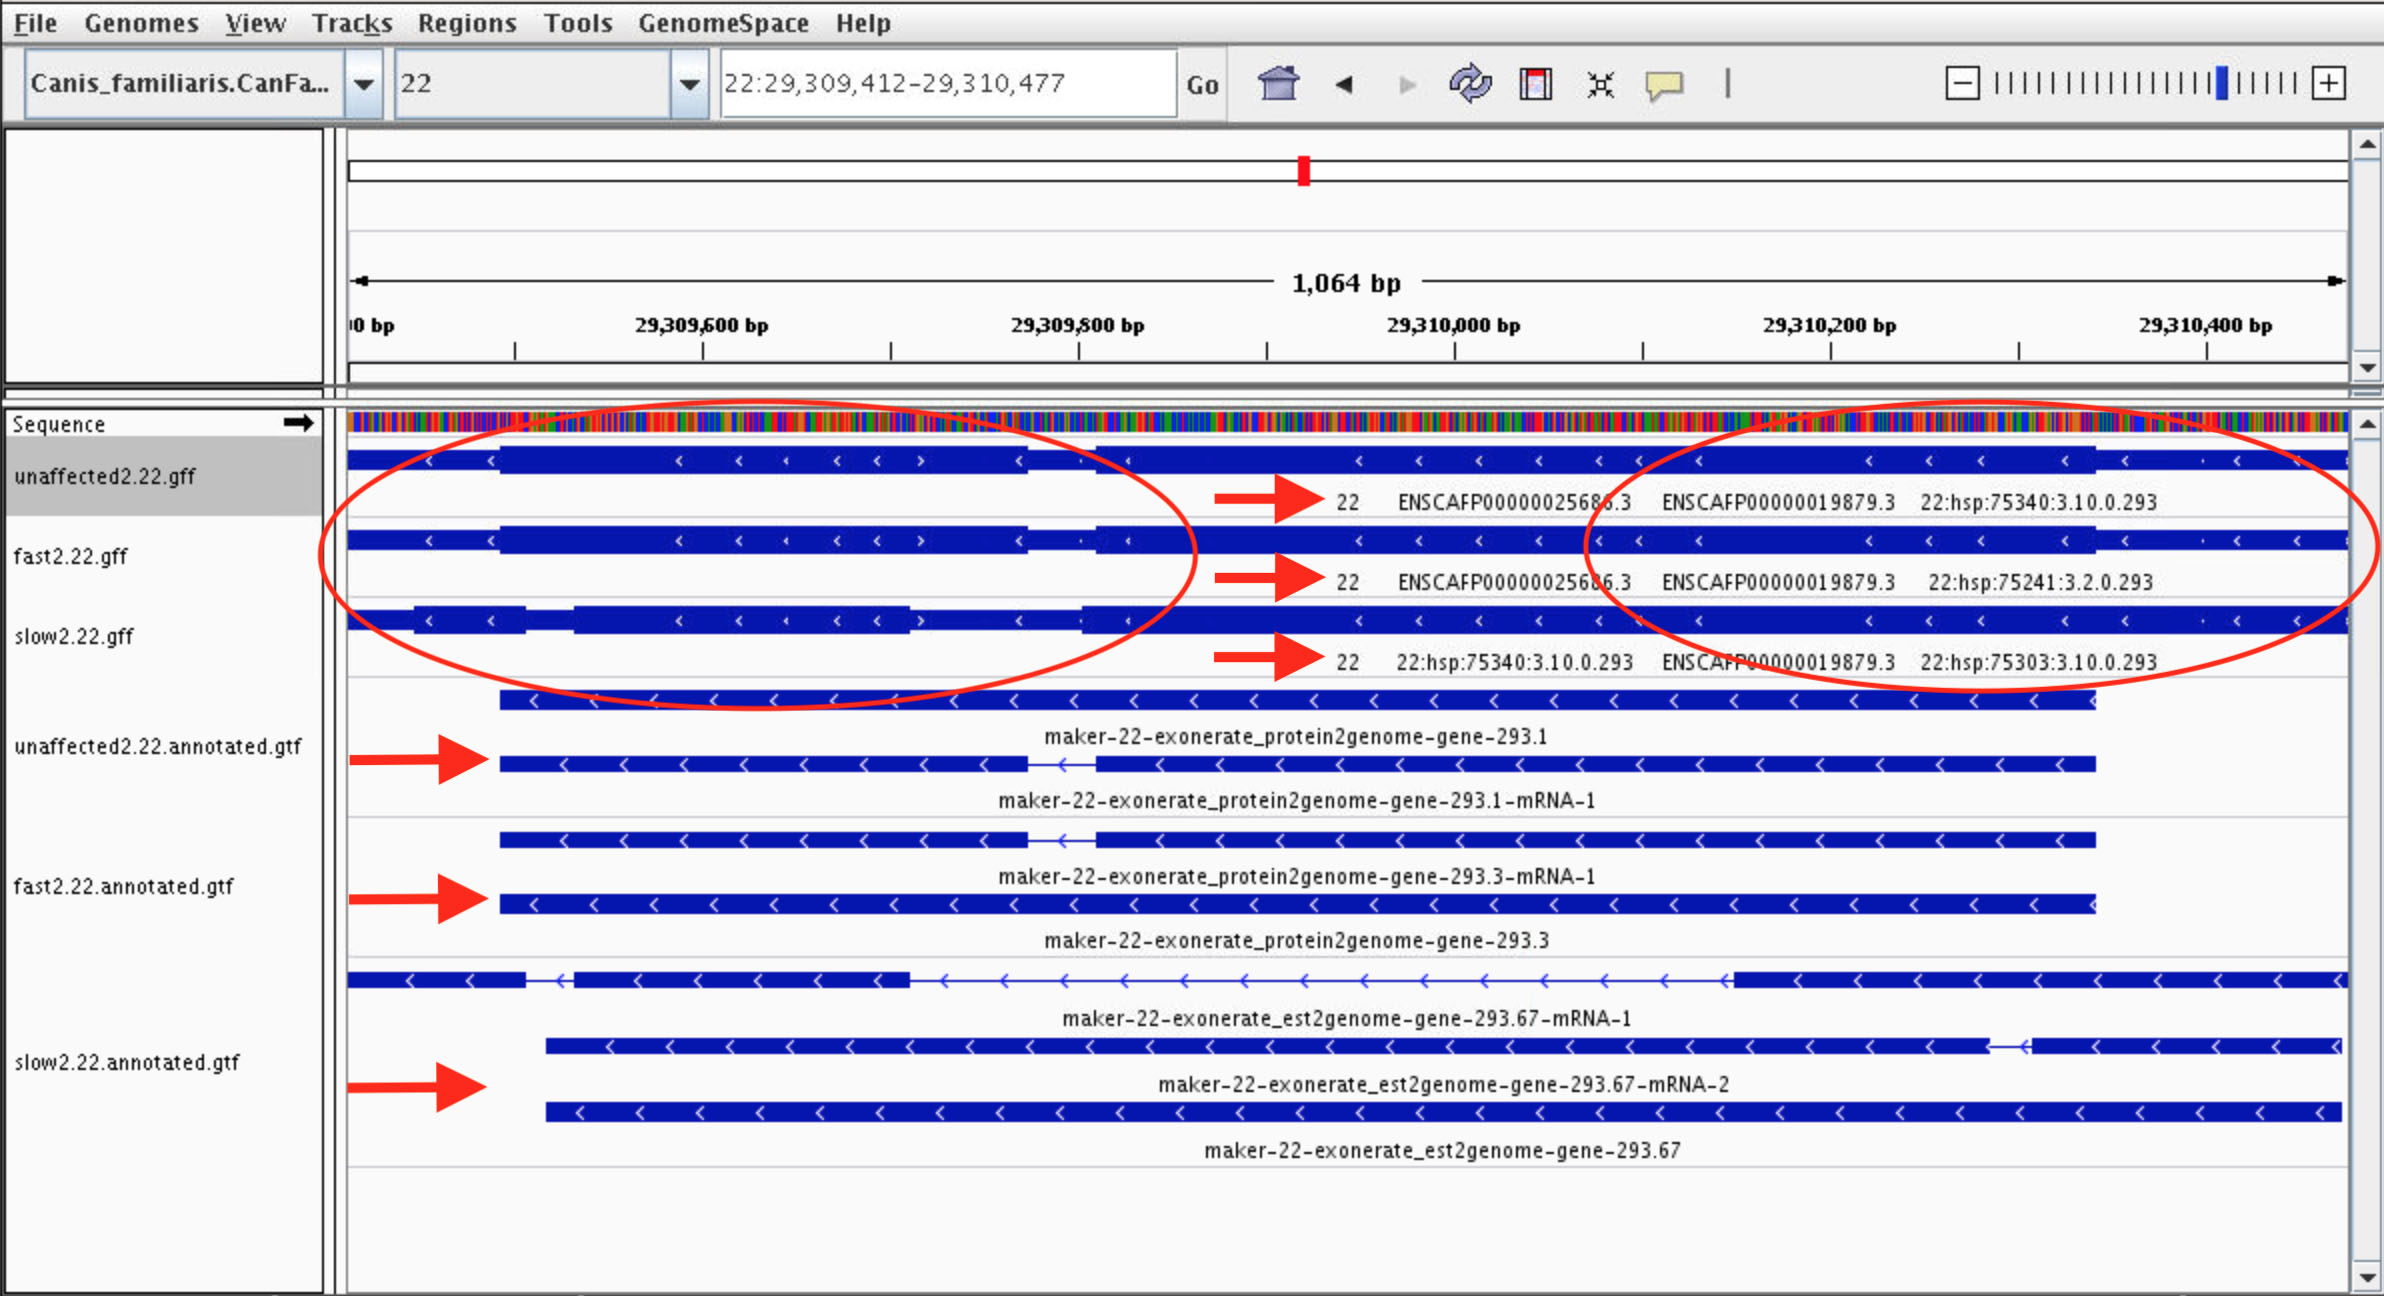
\includegraphics[width=10em]{./IGVGene 1.jpg}}


     \#+CAPTION: gene2 structure slow vs unaffected and fast unaffected
     \#+NAME:   fig: igv$_{\mathrm{gene2\}}$\_{}slow vs unaffected and fast vs unaffected     
     \centerline{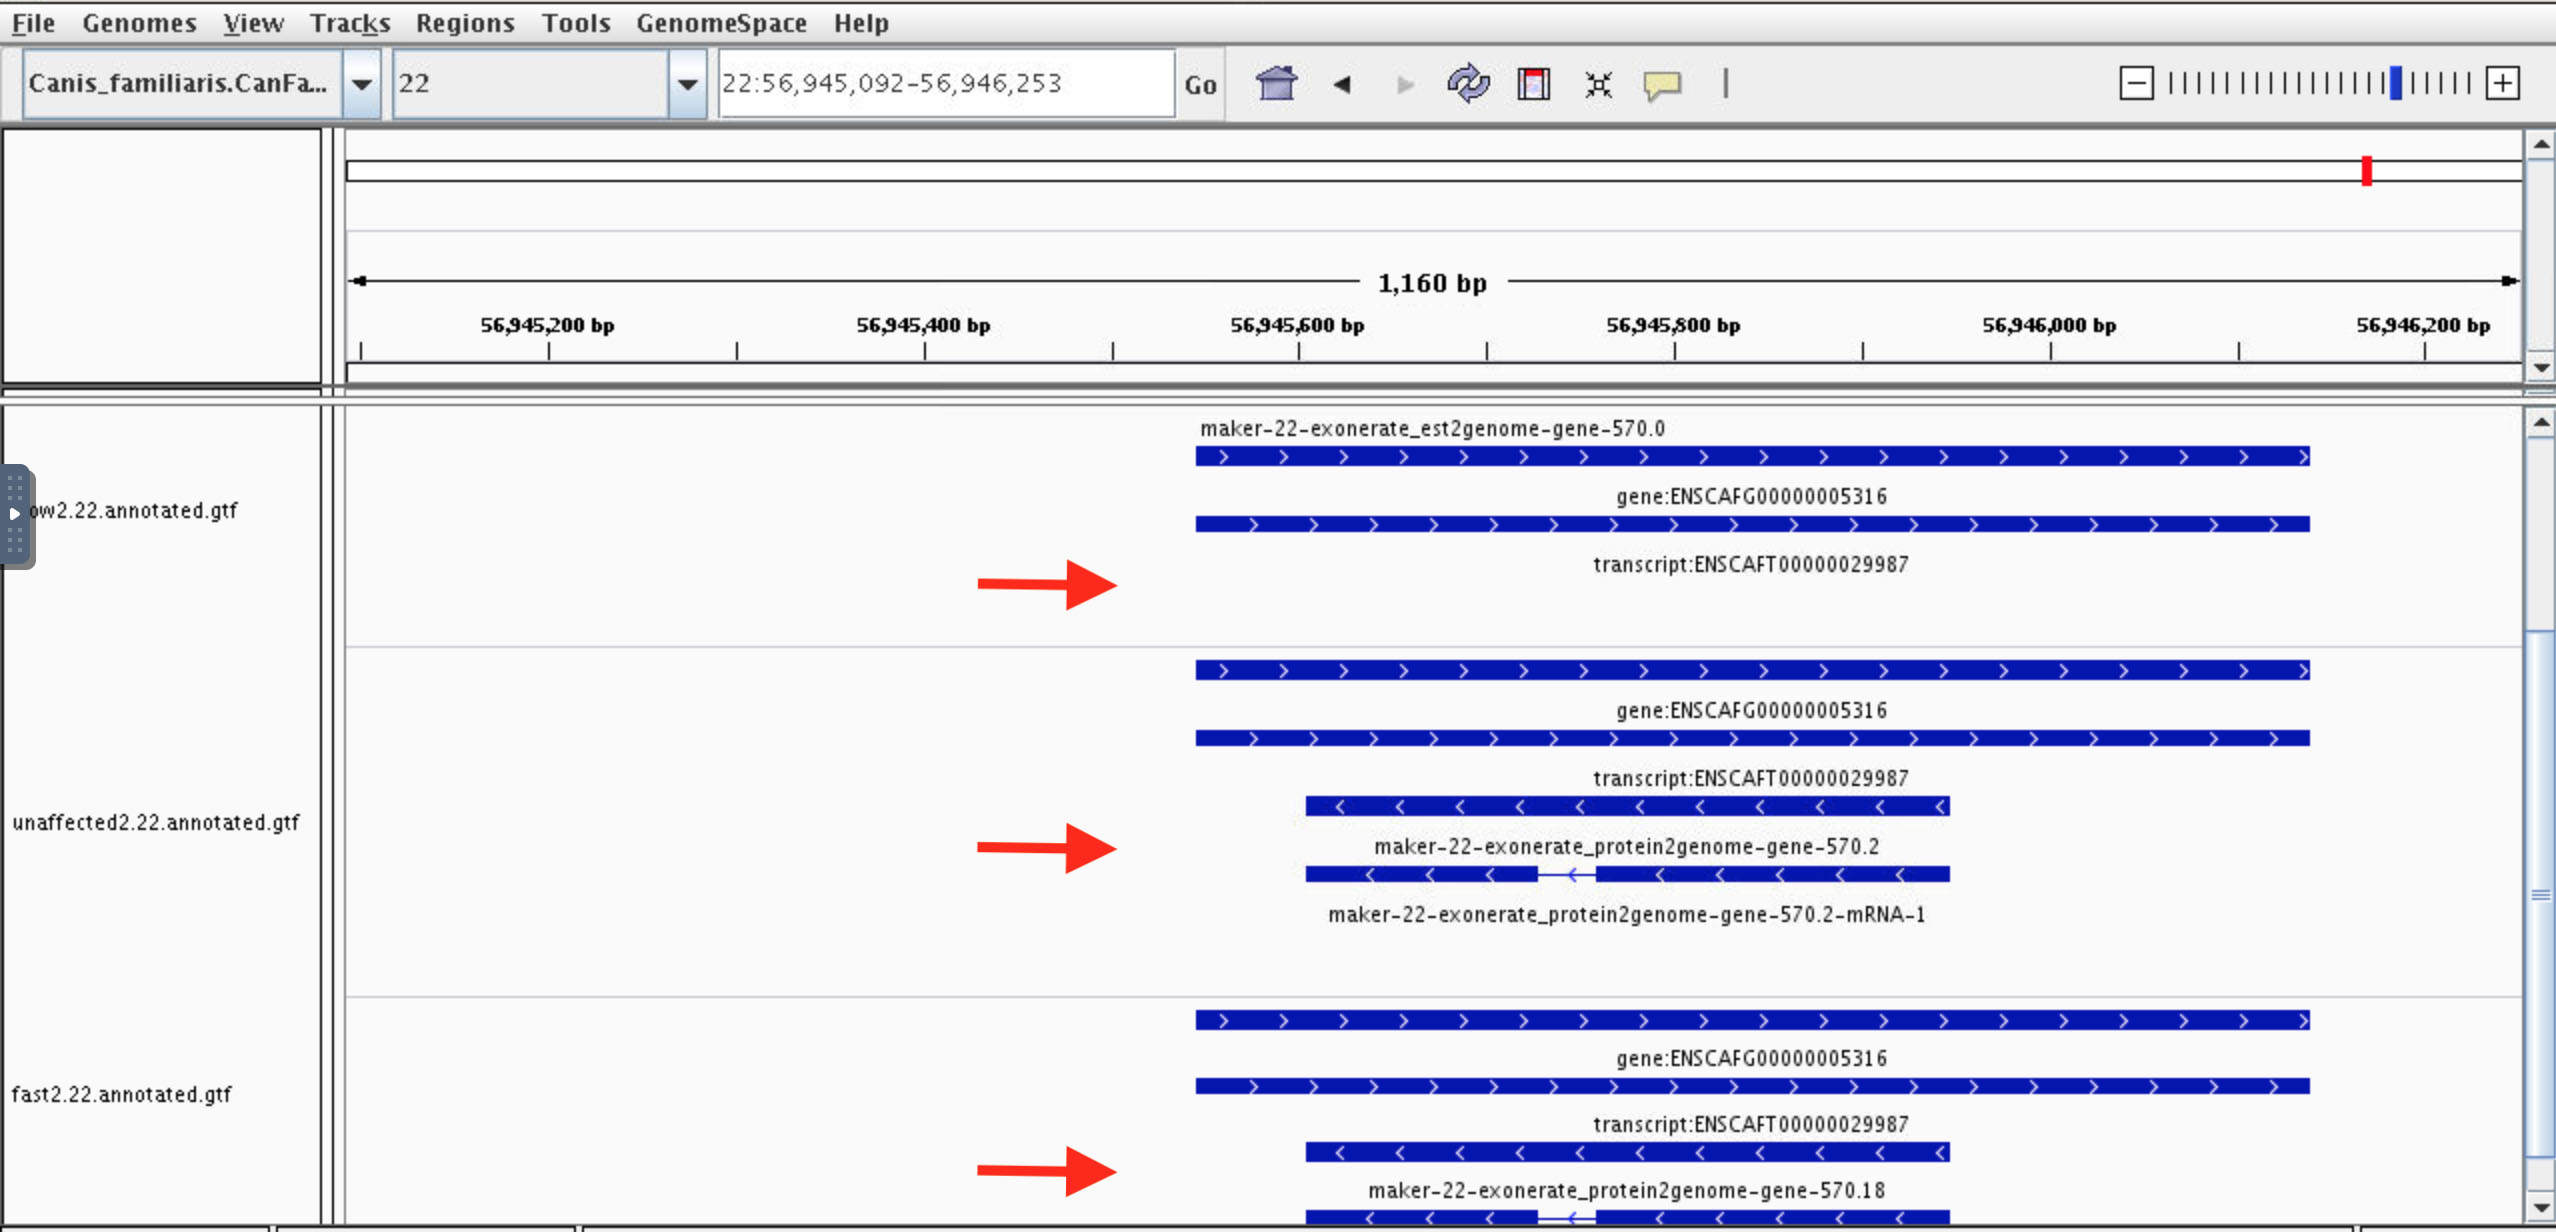
\includegraphics[width=10em]{./IGVGene 2_1.jpg}}

     \centerline{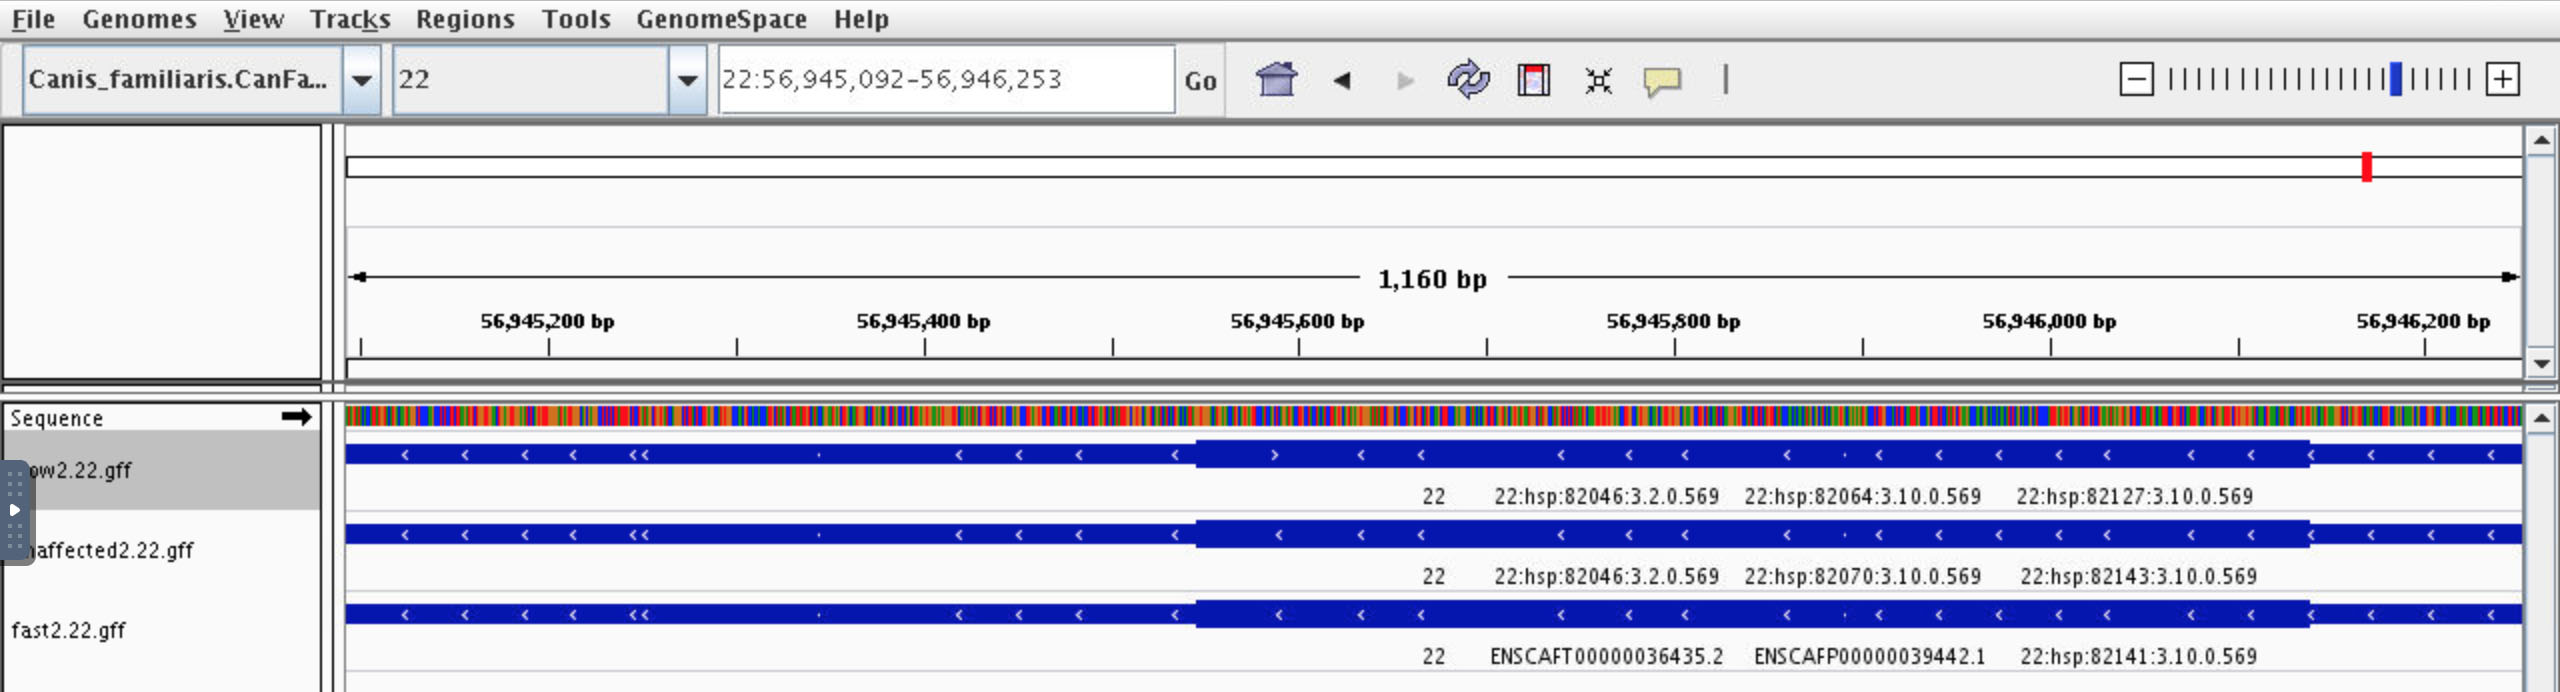
\includegraphics[width=10em]{./IGVGene 2_2.jpg}}
\end{itemize}

\end{itemize}

\item Results (continued)

\begin{itemize}
\item I also extracted the two genes sequences from transcripts file of slow and unaffected condition dogs, and aligned them to check the InDels or SNPs. The results were 
      in accord with IGV observation. There are InDels between slow and unaffected genome for both the two genes. I indicated them with red arrow.

     \#+CAPTION: gene1 alignment slow vs unaffected
     \#+NAME:   fig: gene1 alignment slow vs unaffected
     \centerline{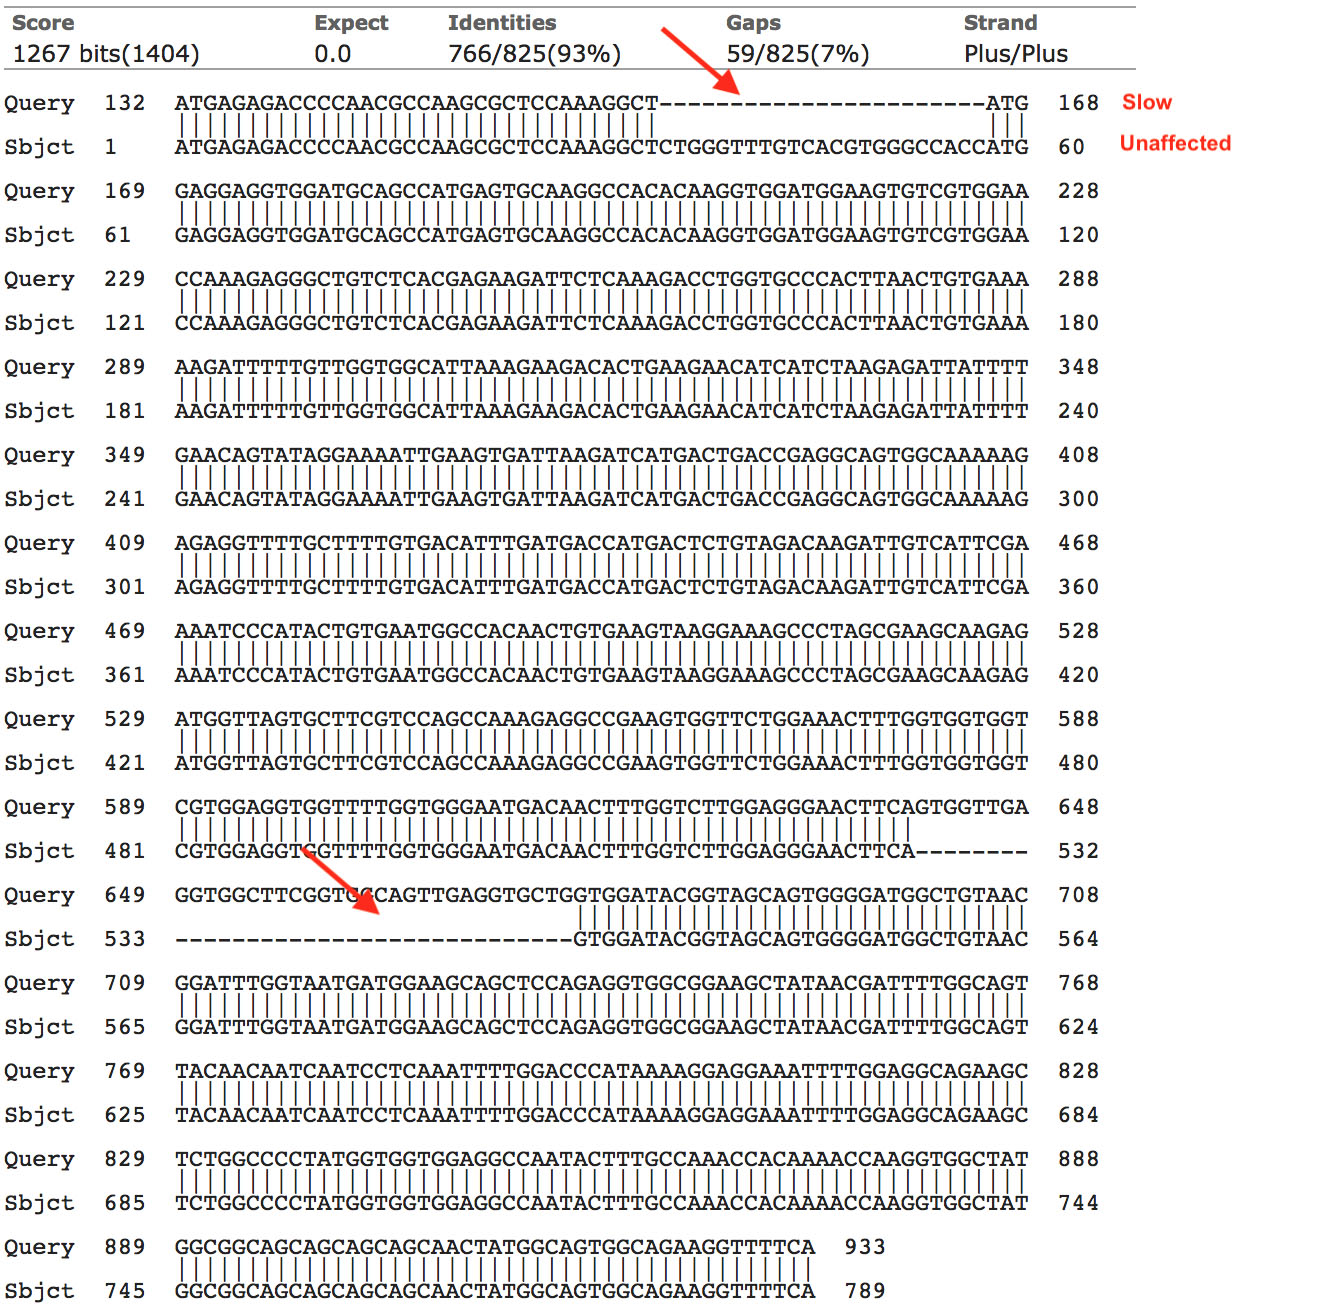
\includegraphics[width=10em]{./alignmentgene1.jpg}}
\end{itemize}

\item Results (continued)

\begin{itemize}
\item I also observed Stringtie files (gtf files), and located in the same chromosome region. But for the first gene, it did not expressed in both unaffected and 
      slow condition dogs. This observation may confirmed the above gffcompare results, which cannot detect the difference between this two conditions based on StringTie
      files. What's more, although the second gene expressed in these two conditions dogs, no difference of gene structure was identified. Importantly,
      I also checked the entire consequence of StringTie GTF files in IGV. I also cannot find any difference of gene structure between the three conditions.
\end{itemize}

\item In summary, I identified that two genes have structure variations between unaffected and slow conditions dogs. After blast, they are mostly like
      HNRNPA1 and GAPDH genes, respectively. Interestingly, these two genes both involved in human neurodegenerative diseases such as amyotrophic lateral sclerosis. 
      Furthermore, the mutation sites in Chromosome22 of dog genome were also identified. The mutation sites involved InDels in slow and 
      unaffected genome for both of the two genes. Probably these mutations (or InDels) in Chromosome 22 are involved with the Duchenne muscular dystrophy (slow condition)
      in dogs.
\item References

\begin{itemize}
\item Cumming, R. C., \& Schubert, D. (2005). Amyloid-β induces disulfide bonding and aggregation of GAPDH in Alzheimer’s disease. The FASEB journal, 19(14), 2060-2062.
\item Tatton, N. A. (2000). Increased caspase 3 and Bax immunoreactivity accompany nuclear GAPDH translocation and neuronal apoptosis in Parkinson's disease. Experimental neurology, 166(1), 29-43.
\item Browne, S. E., Bowling, A. C., Macgarvey, U., Baik, M. J., Berger, S. C., Muquit, M. M., \ldots{} \& Beal, M. F. (1997). Oxidative damage and metabolic dysfunction in Huntington's disease: selective vulnerability of the basal ganglia. Annals of neurology, 41(5), 646-653.
\item Renton, A. E., Chiò, A., \& Traynor, B. J. (2014). State of play in amyotrophic lateral sclerosis genetics. Nature neuroscience, 17(1), 17.
\item Kim, H. J., Kim, N. C., Wang, Y. D., Scarborough, E. A., Moore, J., Diaz, Z., \ldots{} \& Kanagaraj, A. P. (2013). Mutations in prion-like domains in hnRNPA2B1 and hnRNPA1 cause multisystem proteinopathy and ALS. Nature, 495(7442), 467.
\end{itemize}

\end{itemize}

\end{document}
